\documentclass{beamer}
\usepackage[utf8]{inputenc}
\usepackage{graphicx}
\usepackage[croatian]{babel}
\title{KDiff3}
\author{nino.dumicic }
\date{January 2019}

\begin{document}

\maketitle
\begin{frame}{KDiff3}
    
\includegraphics[width=2cm, height=2cm]{kdiff1.png}
    \begin{itemize}
        \item Pokazuje razlike između linija, ali i zasebnih karaktera
        \item Također integriran s Windowsom kao i Tortoise i WinMerge
        \item Integrirani editor za lako riješavanje conflicta
        \item Vlastit log za povijest spajanja
        \item Sučelje slično kao i kod ostalih, no vrlo surovo
    \end{itemize}
\end{frame}
\begin{frame}{Spajanje u KDiff3}
    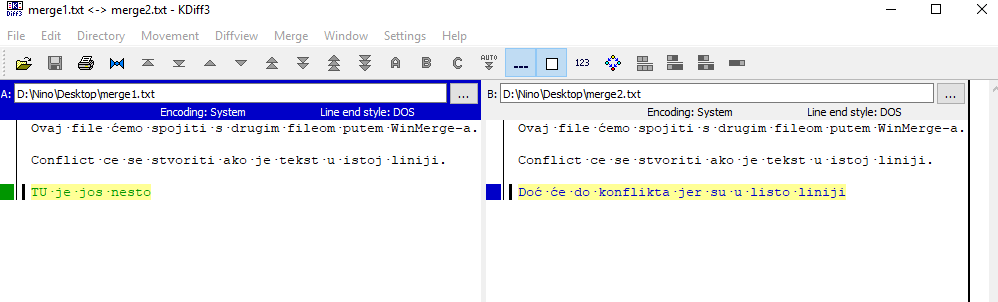
\includegraphics[width=10cm, height=5cm]{kdiff2.png}
    
\end{frame}
    \begin{frame}
    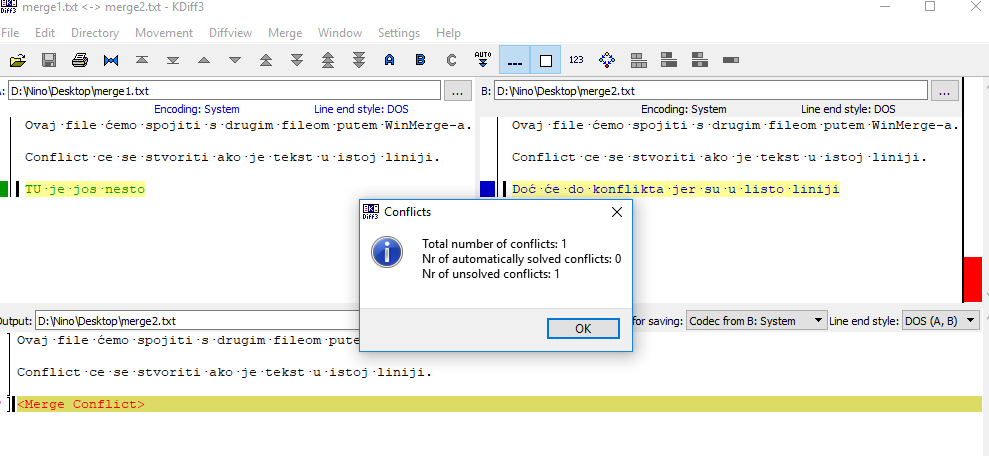
\includegraphics[width=10cm, height=5cm]{kdiff3.png}
    \begin{itemize}
        \item KDiff3 nam točno govori što je mogao riješiti, a što ne u ovom korisnom prozorčiću
    \end{itemize}
    
\end{frame}

\end{document}
